\chapter{Background and Related Work}
\label{ch:background}

The research presented in this thesis lies at the intersection of Internet architecture, network measurements, mobile ecosystems, and the legal frameworks governing international data transfers. In particular, this work focuses on the implications that anycast-based infrastructures have on data protection.

Understanding these implications requires combining knowledge from multiple domains. Firstly, network knowledge about how anycast routing behaves and its internal characteristics is essential. Secondly, knowledge of current data protection regulations related to international transfers of personal data, including the transparency and information obligations imposed on data controllers. Finally, studying the tools and practices, such as the use of TPLs in the Android ecosystem, which is the one used as the case study for this work. Although Android applications are the case study, the knowledge, tools, and regulations apply to all services on the Internet, making it possible to expand this work to other ecosystems like iOS or web services.

\section{Internet Routing and Anycast Communications}
\label{sec:background_internet_routing}

\subsection{Internet Routing Fundamentals}
\label{sc:background_internet_routing_fundamentals}

\begin{figure*}[t]
    \centering
    \begin{tikzpicture}[
    >=Latex,
    font=\small,
    node distance=8mm and 12mm
]

% ============================================================
% PANEL (a)
% ============================================================

\node[
    anchor=west,
    font=\bfseries
] (titlea) at (0,0)
    {(a) Internet routing: geographic distance vs.\ routing path};

% Endpoints
\node[
    endpoint,
    below=7mm of titlea,
    xshift=-65mm
] (sourceA)
    {Source\\(host / AS X)};

\node[
    endpoint,
    right=110mm of sourceA
] (destA)
    {Destination\\(host / AS Y)};

% Autonomous systems
\node[
    autonomoussystem,
    right=10mm of sourceA
] (as1) {AS 1};

\node[
    autonomoussystem,
    right=17mm of as1,
    yshift=10mm
] (as2) {AS 2};

\node[
    autonomoussystem,
    right=17mm of as2
] (as4) {AS 4};

\node[
    autonomoussystem,
    right=17mm of as4,
    yshift=-10mm
] (as5) {AS 5};

% Transit AS
\node[
    autonomoussystem,
    below=15mm of as4
] (as6) {AS 6\\(transit)};

% IXP
\node[
    ixp,
    right=8mm of as2
] (ixp) {IXP};

% Links
\draw[link] (sourceA) -- (as1);
\draw[link] (as1) -- (as2);
\draw[link] (as2) -- (ixp);
\draw[link] (ixp) -- (as4);
\draw[link] (as4) -- (as5);
\draw[link] (as5) -- (destA);

% Transit path
\draw[transit] (as1) -- (as6);
\draw[transit] (as6) -- (as5);

% Actual BGP-selected path
\draw[bgppath] (as1) -- (as2);
\draw[bgppath] (as2) -- (ixp);
\draw[bgppath] (ixp) -- (as4);
\draw[bgppath] (as4) -- (as5);

% Geographic shortest path
\draw[shortest]
    (sourceA.north east)
    .. controls
        +(25mm,12mm)
        and +(-25mm,12mm)
    ..
    (destA.north west);

\node[
    text=green!45!black,
    font=\footnotesize\bfseries,
    align=center
] at (
    $(sourceA.north)!0.5!(destA.north)+(0,15mm)$
)
{
    Geographically shortest path\\
    (not necessarily used)
};

\node[
    text=blue!80!black,
    font=\footnotesize\bfseries,
    align=center
] at (
    $(as2.south)!0.5!(as4.south)+(0,-9mm)$
)
{
    Actual routing path selected by BGP\\
    based on policies, peering, and traffic engineering
};

% ============================================================
% Key concepts box
% ============================================================

\node[
    draw,
    rounded corners=3pt,
    fill=blue!3,
    text width=61mm,
    align=left,
    inner sep=5pt,
    font=\footnotesize
] at (
    $(sourceA.south)!0.5!(as6.south)+(-2mm,-17mm)$
)
{
    \textbf{Key concepts}
    \begin{itemize}
        \setlength{\itemsep}{1pt}
        \setlength{\parskip}{0pt}
        \item Internet routing (e.g., BGP) selects paths according
        to routing policies, not physical distance.
        
        \item Peering relationships and traffic engineering may
        lead to longer geographic paths.
        
        \item Network proximity does not necessarily imply
        geographic proximity.
    \end{itemize}
};

% Separator
\draw[
    gray!50,
    line width=0.7pt
] (-88mm,-67mm) -- (88mm,-67mm);

% ============================================================
% PANEL (b)
% ============================================================

\node[
    anchor=west,
    font=\bfseries
] (titleb) at (-88mm,-73mm)
{
    (b) Anycast routing: one IP, multiple geographically
    distributed replicas
};

% Source
\node[
    endpoint,
    below=7mm of titleb,
    xshift=-65mm
] (sourceB)
    {Source\\(host / AS X)};

% ASes
\node[
    autonomoussystem,
    right=10mm of sourceB
] (bas1) {AS 1};

\node[
    autonomoussystem,
    right=17mm of bas1,
    yshift=10mm
] (bas2) {AS 2};

\node[
    autonomoussystem,
    right=17mm of bas2
] (bas4) {AS 4};

\node[
    autonomoussystem,
    right=17mm of bas4,
    yshift=-10mm
] (bas5) {AS 5};

% IXP
\node[
    ixp,
    right=8mm of bas2
] (bixp) {IXP};

% Anycast IP
\node[
    anycastip,
    right=12mm of bas5
] (ip)
{
    Anycast IP\\
    \texttt{203.0.113.1}
};

% Replicas
\node[
    replica,
    right=16mm of ip,
    yshift=13mm
] (r1)
{
    Replica 1\\
    Madrid, Spain
};

\node[
    replica,
    right=16mm of ip
] (r2)
{
    Replica 2\\
    Paris, France
};

\node[
    replica,
    right=16mm of ip,
    yshift=-13mm
] (r3)
{
    Replica 3\\
    New York, USA
};

% Links
\draw[link] (sourceB) -- (bas1);
\draw[link] (bas1) -- (bas2);
\draw[link] (bas2) -- (bixp);
\draw[link] (bixp) -- (bas4);
\draw[link] (bas4) -- (bas5);
\draw[link] (bas5) -- (ip);

% Selected routing path
\draw[bgppath]
    (bas1) -- (bas2)
    -- (bixp)
    -- (bas4)
    -- (bas5);

% Anycast replicas
\draw[replicaLink] (ip) -- (r1);
\draw[replicaLink] (ip) -- (r2);
\draw[replicaLink] (ip) -- (r3);

% Replica annotation
\node[
    align=left,
    font=\footnotesize
] at (
    $(r2.east)+(20mm,0)$
)
{
    Multiple replicas\\
    sharing the same\\
    anycast IP address
};

% ============================================================
% Anycast principle box
% ============================================================

\node[
    draw,
    rounded corners=3pt,
    fill=violet!3,
    text width=68mm,
    align=left,
    inner sep=5pt,
    font=\footnotesize
] at (
    $(sourceB.south)!0.5!(bas5.south)+(-2mm,-18mm)$
)
{
    \textbf{Anycast principle}
    \begin{itemize}
        \setlength{\itemsep}{1pt}
        \setlength{\parskip}{0pt}
        \item Multiple geographically distributed replicas share
        the same IP address.
        
        \item Routing protocols deliver packets to the replica
        selected according to routing policies and current
        network conditions.
        
        \item The selected replica, and therefore the geographic
        destination, may vary across sources and over time.
    \end{itemize}
};

\end{tikzpicture}

    \caption{From Internet routing to anycast.(a) Internet routing decisions are influenced by routing policies, peering relationships, and traffic engineering, and therefore the selected path does not necessarily correspond to the geographically shortest path. (b) Anycast allows multiple geographically distributed replicas to share the same IP address. The routing system selects one of these replicas according to the routing conditions observed from the source, so the actual geographic destination may vary across sources and over time.}
    \label{fig:internet-routing-anycast}
\end{figure*}

The Internet is composed of thousands of interconnected Autonomous Systems (ASes) that exchange reachability information using BGP. Each AS independently applies routing policies according to business relationships, traffic engineering objectives, operational constraints, and security considerations. Consequently, Internet routing decisions are not exclusively determined by shortest-path metrics but by a highly dynamic combination of economic, administrative, and topological factors.

BGP operates as a policy-based path-vector protocol in which routes are selected based on multiple attributes, including AS path length, local preference, routing policies, and peering agreements. For example, peering agreements may involve direct interconnections established through private links or Internet Exchange Points, creating connectivity that is not explicitly visible at the IP layer and allowing a single IP hop to span large geographic distances. As a result, the path selected between two endpoints may not correspond to the geographically shortest route. Instead, routing decisions are frequently optimised according to operational or economic objectives such as minimising transit costs, balancing traffic loads, or improving resilience.

This behaviour becomes particularly relevant in large-scale distributed infrastructures, where routing dynamics may significantly affect the geographic path followed by user communications. Phenomena such as traffic engineering, route aggregation, or peering asymmetries may cause communications to traverse jurisdictions that are geographically distant from the user or from the intended service region.

Traditionally, Internet communications followed a unicast paradigm in which a destination IP address uniquely identifies a single host or service instance. Under this model, the logical destination of a communication can generally be associated with a relatively stable physical location, allowing organisations and users to reason about where communications are being processed.

However, modern Internet infrastructures increasingly rely on distributed service architectures in order to improve scalability, resilience, fault tolerance, and latency. Services such as CDNs, authoritative DNS providers, cloud platforms, and DDoS mitigation systems deploy geographically distributed replicas of the same service across multiple locations worldwide. To efficiently redirect traffic towards these distributed replicas, many of these systems rely on anycast addressing.

These properties have made anycast a fundamental building block of the modern Internet \cite{Abley2006OperationServices,McPherson2014ArchitecturalAnycast}, but they also create significant challenges for privacy, auditing, and regulatory compliance. Understanding how anycast routing interacts with geographic control mechanisms is therefore essential for analysing the privacy implications addressed throughout this thesis.

\subsection{Anycast Routing}
\label{sc:background_internet_routing_anycast}

Anycast routing is not a recent concept. The first references to anycast services appeared in RFC 1546 in 1993 \cite{Partridge1993HostService}. Later, anycast addressing was formally incorporated into the IPv6 architecture specification \cite{Hinden2003InternetArchitecture}, while ICMPv6 introduced specific operational considerations for anycast communications \cite{Conta2006InternetSpecification}.

According to the IPv6 specification, an anycast address is defined as:

\begin{quote}
An anycast address is an address that is assigned to more than one interface (typically belonging to different nodes), with the property that a packet sent to an anycast address is routed to the "nearest" interface having that address, according to the routing protocols' measure of distance. \cite{Hinden2003InternetArchitecture}
\end{quote}
Anycast
Unlike unicast communications, where an IP address maps to a single destination, anycast allows multiple geographically distributed nodes to share the same IP address. Routing protocols then determine which replica receives a given communication according to topological distance and routing policies.

This decoupling between logical addressing and physical location constitutes one of the key characteristics of anycast systems. While it enables substantial improvements in scalability and resilience, it also introduces important challenges regarding transparency, geographic determinism, and control over data flows. In particular, the actual physical destination of a communication may dynamically change over time depending on routing updates, network congestion, failures, or operational policies.

Despite these advantages, anycast introduces a major limitation: the physical destination of a communication becomes non-deterministic from the perspective of end users and applications. The actual server instance reached by a communication depends on dynamic BGP decisions, peering relationships, traffic engineering policies, routing failures, and network conditions.

Consequently, two users located in the same country may reach infrastructures deployed in different jurisdictions. Similarly, a communication initially routed towards a nearby region may later be redirected to another country due to routing changes or operational events. This behaviour creates important challenges regarding transparency, auditing, and geographic control of personal data flows.

Furthermore, previous works have shown that anycast routing behaviour may significantly differ from geographic proximity assumptions \cite{Bian2019TowardsPeering,Calder2015AnalyzingCDN}. In practice, the topologically nearest node does not necessarily correspond to the geographically closest infrastructure.

\subsection{Anycast in Modern Internet Services}
\label{sc:background_internet_routing_anycast_modern}

The deployment of anycast infrastructures has grown substantially over the last year. Today, some of the most critical Internet services rely on anycast as a core architectural mechanism.

\begin{figure}[h]
    \centering
    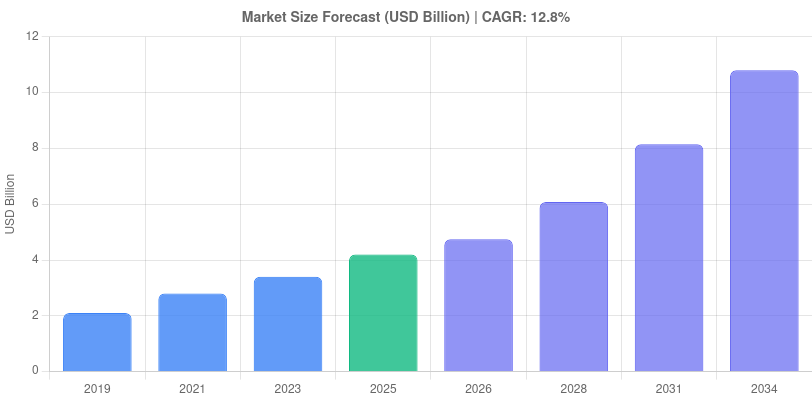
\includegraphics[width=\textwidth]{figures/images/anycast_market_size_2019-2034.png}
    \caption{Anycast Network Services Market Size 2019 - 2034 \cite{Anycast2034}.}
    \label{fig:hunter_traceroute_protocols_examples}
\end{figure}

\subsubsection{Content Delivery Networks}
\label{sc:background_internet_routing_anycast_modern_cdns}

CDNs distribute content across globally distributed infrastructures in order to reduce latency and improve user experience. Large CDNs extensively employ anycast to redirect users towards nearby edge servers \cite{Calder2015AnalyzingCDN}. These systems continuously optimise routing decisions according to traffic demand, congestion, and infrastructure availability.

Although CDN architectures improve scalability and performance, they also introduce important privacy implications. Previous work has investigated privacy-preserving CDN architectures and the risks associated with information leakage through user requests and content access patterns \cite{Cui2020Multi-CDN:Networks,Vo2025OblivCDN:Access}. These studies focus primarily on protecting the confidentiality of communications and preventing content providers or CDN operators from inferring sensitive information about users. User requests may also traverse multiple jurisdictions depending on routing dynamics, cache placement strategies, or traffic balancing policies. In contrast, this thesis addresses privacy and data protection from a geographic perspective, analysing how distributed infrastructures and routing decisions influence the jurisdictions where communications are processed and the implications that such behaviour may have for international data transfers and geographic control.

\subsubsection{DNS Infrastructures}
\label{sc:background_internet_routing_anycast_modern_dns}

The Domain Name System (DNS) represents one of the earliest large-scale adopters of anycast. Root DNS servers and authoritative DNS providers commonly use anycast to improve availability and resilience against attacks \cite{Abley2006OperationServices}.

However, DNS communications may reveal sensitive information regarding users' browsing activities, accessed domains, or application behaviours. Previous work has extensively studied the privacy implications of DNS and proposed mechanisms aimed at protecting the confidentiality of DNS queries and mitigating information leakage \cite{Bortzmeyer2015DNSConsiderations, Hu2023CharacterizingTraffic}. These efforts primarily focus on preventing recursive resolvers, network operators, or external observers from inferring sensitive information from DNS traffic. Nevertheless, the geographic destination of DNS queries also has important implications for privacy and surveillance, as queries may be processed in jurisdictions different from those expected by users or service providers. In contrast to previous work focused on the confidentiality of DNS communications, this thesis addresses their geographic dimension and analyses the implications that distributed infrastructures and routing dynamics have for international data transfers and geographic control.

\subsubsection{Cloud and DDoS Mitigation Services}
\label{sc:background_internet_routing_anycast_modern_ddos}

Cloud providers and anti-DDoS platforms increasingly rely on anycast infrastructures to absorb large traffic volumes and provide globally distributed protection services. These architectures allow malicious traffic to be distributed across multiple scrubbing centres.

Nevertheless, the geographic dispersion of these infrastructures complicates the determination of where user traffic is actually processed. In many cases, users and organisations are unaware of the jurisdictions involved in the communication path.

\section{Geographic Location and Internet Measurements}
\label{sc:background_location_measurements}

\subsection{IP Geolocation}
\label{sc:background_location_measurements_ip_geolocation}

Determining the geographic location of Internet hosts is a long-standing challenge in network research. Existing IP geolocation techniques can generally be classified into database-based approaches and measurement-based approaches.

Database-based systems rely on information collected from RIRs, WHOIS records, commercial datasets, routing announcements, or infrastructure metadata. However, previous works have demonstrated that these databases frequently contain outdated, coarse-grained, or inaccurate information \cite{Ding2015AnSub-networks, Dan2021IPInterpolation, Cozar2022ReliabilityTransfers}.

Measurement-based approaches attempt to infer geographic location through active network measurements such as latency estimation, traceroute analysis, or landmark-based triangulation \cite{Cicalese2015AGeolocation,Cicalese2016Latency-BasedSets,Ciavarrini2018GeolocationBound}. These approaches often provide better accuracy, particularly when estimating the location of distributed infrastructures, at the cost of multiple measurements for every desired result.

The work presented in this thesis builds upon these measurement-based approaches to estimate the geographic destinations of anycast communications. However, anycast introduces additional complexity because the same IP address may correspond to multiple geographically distributed replicas.

\subsection{Traceroute and Path Inference}
\label{sc:background_location_measurements_pathing}

Traceroute-based methodologies constitute one of the most widely used techniques for studying Internet routing behaviour. By analysing intermediate routers and round-trip times, traceroute allows researchers to estimate routing paths and infer topological properties of the network.

Nevertheless, traceroute measurements suffer from multiple limitations, including:

\begin{itemize}
    \item \textbf{ICMP filtering}: routers or firewalls block or rate-limit ICMP messages, preventing some hops from responding.
    \item \textbf{Asymmetric routing}: forward and return paths may differ.    
    \item \textbf{MPLS tunnels}: packet forwarding through MPLS networks hides intermediate routers or alters the topology observed by traceroute.
    \item \textbf{Load balancing}: packets belonging to the same traceroute follow different paths, leading to inconsistent or variable measurements.
    \item \textbf{Hidden routers}: some routers are configured not to generate ICMP responses.
    \item \textbf{Dynamic routing changes}: routing decisions change during measurements due to network events or traffic engineering policies, producing unstable paths.
\end{itemize}

Previous studies have analysed these limitations and proposed techniques to improve path inference accuracy \cite{Dainotti2012IssuesClassification}. In the context of anycast, traceroute measurements become even more challenging because routing paths may dynamically change between measurements, and different replicas may respond with the same destination IP address.

\subsection{Latency-Based Geolocation}
\label{sc:background_location_measurements_latency_geolocation}

Latency-based geolocation techniques estimate geographic distance from network delay measurements. Since signal propagation speed imposes physical limits on communication latency, Round Trip Time (RTT) measurements can be used to infer approximate geographic regions.

Several works have explored the use of multilateration and landmark-based systems to estimate IP locations \cite{Cicalese2015AGeolocation, Cicalese2016Latency-BasedSets}. More recent approaches incorporate probabilistic models and large-scale measurement infrastructures \cite{Kohls2022VerLoc:Systems, Sommese2020MAnycast2:Anycast}.

This thesis leverages these concepts to estimate the likely geographic destination of anycast communications using distributed probing infrastructures and latency constraints.

\subsection{Internet Measurement Infrastructures}
\label{sc:background_location_measurements_infraestructures}

Many network measurements can theoretically be performed from a single host. However, such an approach severely limits the geographic diversity of the observations, since all measurements originate from a fixed location. The study of Internet routing, latency, topology, and geographic behaviour often requires measurements from multiple distributed vantage points capable of observing the network under different conditions.

Several large-scale measurement infrastructures have been developed to support Internet research and operational studies. Examples include Ark CAIDA \cite{ArkCAIDA}, perfSONAR \cite{PerfSONAR}, and PlanetLab \cite{HomePlanetLab}. These platforms provide different levels of visibility and measurement capabilities, supporting a wide variety of networking studies.

Among the currently available infrastructures, RIPE Atlas \cite{HomeAtlas} has become one of the most widely adopted platforms for Internet measurements. RIPE Atlas is a large-scale Internet measurement platform composed of thousands of probes and anchors distributed worldwide. These devices are hosted by volunteers, Internet Service Providers (ISPs), universities, research institutions, and organisations, providing broad visibility into the operational Internet from a diverse set of networks and geographic locations.

RIPE Atlas supports a variety of active measurements, including ping, traceroute, DNS, TLS, HTTP, and NTP queries. Measurements can be executed on demand or scheduled periodically, enabling both short-term experiments and long-term monitoring campaigns. The platform is publicly accessible and community-driven, allowing participants to contribute probes and perform measurements through a credit-based system.

The platform is maintained by the RIPE Network Coordination Centre (RIPE NCC), the Regional Internet Registry responsible for Europe, the Middle East, and parts of Central Asia. As one of the organisations involved in Internet coordination and infrastructure management, RIPE NCC provides a reliable and widely adopted platform that has become a de facto standard for Internet-scale measurement studies.

The availability of geographically distributed vantage points makes platforms such as RIPE Atlas particularly valuable for studies involving routing behaviour, latency analysis, geolocation, and anycast infrastructures. Consequently, RIPE Atlas has been extensively employed in research addressing Internet topology, traffic engineering, geographic inference, and the characterisation of distributed services.

\section{Measurement Infrastructure}
\label{sc:hunter_measurement_infrastructure}

The network measurements described in the previous sections could theoretically be performed from a single personal computer. However, such an approach would severely limit the geographic diversity of the measurements, since the location of the measurement host would remain fixed. As the objective of Hunter is to infer the potential geographic destinations of anycast communications on a continental and global scale, it is necessary to employ a distributed measurement infrastructure that provides geographically diverse vantage points.

For this purpose, the implementation of Hunter relies on RIPE Atlas \cite{HomeAtlas}, a large-scale Internet measurement platform composed of thousands of distributed probes deployed worldwide. RIPE Atlas enables researchers and network operators to perform active measurements such as ping, traceroute, DNS, TLS, HTTP, and NTP from multiple geographic locations. These probes are hosted by volunteers, organisations, universities, Internet Service Providers (ISPs), and research institutions, providing broad visibility into the global Internet infrastructure.

The platform is publicly accessible and community-driven, allowing participants to contribute probes and perform measurements through a credit-based system. RIPE Atlas is maintained by the RIPE Network Coordination Centre (RIPE NCC), the Regional Internet Registry responsible for Europe, the Middle East, and parts of Central Asia. As one of the major organisations involved in Internet coordination and infrastructure management, RIPE NCC provides a reliable and widely adopted platform for Internet-scale measurement studies.

Several alternative Internet measurement platforms exist, including Ark CAIDA \cite{ArkCAIDA}, perfSONAR \cite{PerfSONAR}, and PlanetLab \cite{HomePlanetLab}. However, RIPE Atlas was selected for this work due to its large number of active probes, extensive geographic coverage, measurement flexibility, and widespread adoption within the network research community.

These characteristics make RIPE Atlas particularly suitable for the objectives of Hunter, as the method requires executing traceroute and latency measurements from multiple distributed vantage points in order to estimate the geographic regions that are potentially reachable by anycast communications.

\section{Privacy, Data Sovereignty, and International Data Transfers}
\label{sc:background_privacy}

\subsection{Privacy Regulations}
\label{sc:background_privacy_regulations}

Over the last decade, privacy and data protection regulations have become increasingly strict worldwide. Regulations such as the General Data Protection Regulation (GDPR) \cite{REGULATIONSRelevance}, the Data Protection Act from UK \cite{Data2018}, the Australian Privacy Principles \cite{ReadOAIC}, and China's Personal Information Protection Law \cite{TheTranslation} establish obligations regarding transparency, user consent, and international data transfers. In the case of GDPR, Article 13 requires data controllers to inform data subjects when personal data may be transferred to a third country or international organisation, including the legal basis and safeguards applicable to such transfers. Consequently, organisations must not only ensure that international transfers comply with the regulatory requirements established in Chapter V of the GDPR, but also provide accurate information regarding the jurisdictions where personal data may be processed.

A common aspect shared by these regulations is the requirement that organisations maintain control over where personal data is processed and transferred. In many jurisdictions, transfers to foreign countries are only permitted under specific safeguards, adequacy decisions, or contractual mechanisms.

\hugo{Review this sentence, IA suggested}The Court of Justice of the European Union (CJEU) Schrems II ruling significantly reinforced concerns regarding international data transfers by invalidating the EU-US Privacy Shield framework. This decision increased the importance of understanding where personal data is actually routed and processed.

In parallel, governments and regulatory agencies have progressively emphasised the importance of transparency obligations. Organisations are often required to disclose not only what personal data is collected but also the entities involved in their processing, the purposes of the processing activities, and the countries to which the data may be transferred. However, these transparency requirements implicitly assume that organisations possess sufficient knowledge and control over the geographic behaviour of their infrastructures.

This assumption becomes problematic in highly distributed Internet architectures. Modern services frequently rely on complex chains of providers, including cloud infrastructures, CDNs, anti-DDoS systems, analytics services, and third-party APIs. Many of these systems internally employ anycast routing and globally distributed deployments, making the actual destination of communications highly dynamic and difficult to predict.

Consequently, even organisations operating under strict regulatory frameworks may unintentionally trigger international data transfers that are not accurately reflected in their privacy policies or internal compliance procedures. This situation creates a mismatch between legal expectations regarding geographic control and the operational realities of Internet-scale infrastructures.

\subsection{Data Sovereignty}
\label{sc:background_privacy_data_sovereignty}

Data sovereignty refers to the principle that digital information is subject to the laws and governance structures of the jurisdiction where it is stored or processed. The concept has become increasingly relevant as governments attempt to regulate the flow of digital information across borders and reduce dependence on foreign infrastructures.

Traditionally, data sovereignty discussions focused primarily on storage location. Under this perspective, organisations could maintain geographic control by selecting data centres deployed within specific jurisdictions. However, modern distributed architectures challenge this simplified view because communications and processing operations may dynamically traverse multiple countries, even when the primary infrastructure appears to be regionally constrained.

Anycast infrastructures further complicate this scenario. Since multiple geographically distributed replicas share the same IP address, the geographic destination of a communication may change over time depending on routing dynamics, network conditions, or operational policies. As a result, geographic assumptions based solely on administrative configurations or provider declarations may not accurately represent the actual path followed by user data.

This issue is particularly relevant in environments where legal obligations require strict regionalisation of communications. For example, organisations operating under GDPR may attempt to ensure that European user data remains within the European Economic Area. Nevertheless, if communications are routed through anycast infrastructures operated by globally distributed providers, data may transiently or permanently traverse non-European jurisdictions without explicit awareness from either users or service operators.

Moreover, data sovereignty concerns extend beyond regulatory compliance. Geographic routing decisions may expose communications to different surveillance frameworks, intelligence collection programmes, or national security legislation depending on the countries involved in the communication path. Therefore, understanding where communications are actually routed becomes a fundamental requirement not only for compliance purposes but also for broader privacy and trust considerations.

\subsection{International Data Transfers in Distributed Infrastructures}
\label{sc:background_privacy_international_data_transfers}

International data transfers are inherent to the operation of the modern Internet. Cloud computing platforms, CDN infrastructures, and mobile ecosystems continuously exchange information across multiple geographic regions in order to provide scalability, redundancy, and low latency services. While distributed architectures provide substantial technical benefits, they also complicate the identification of where personal data is processed at any given moment. In practice, communications may involve numerous intermediate entities, including DNS providers, CDN edge servers, authentication platforms, telemetry systems, and advertisement infrastructures.

This complexity is further amplified in mobile environments. Modern applications rarely communicate exclusively with infrastructures controlled by the application developer. Instead, they interact with multiple third-party services integrated through Software Development Kits (SDKs) and TPLs. Each of these external dependencies may independently establish communications with globally distributed infrastructures. As a consequence, a single user action performed within a mobile application may trigger multiple parallel communications involving several countries and service providers. These communications are often opaque to users and difficult to audit from the perspective of developers or organisations.

Several studies have demonstrated that privacy disclosures frequently fail to provide accurate information regarding such complex data-sharing ecosystems \cite{DelAlamo2021PrivacyStudy, DelAlamo2022APolicies}. However, most previous analyses focus on organisational relationships and declared third parties rather than on the actual network-level geographic behaviour of communications.

This thesis extends prior work by analysing international data transfers from a network-layer perspective. Instead of exclusively studying contractual or declarative aspects, this work investigates where communications are physically routed when anycast infrastructures participate in the delivery process.

\subsection{Geographic Transparency Limitations}
\label{sc:background_privacy_transpanency}

\hugo{Include more examples of bad practices.} Current transparency mechanisms are generally insufficient to accurately describe the geographic behaviour of modern distributed systems. Privacy policies commonly provide high-level descriptions, such as "data may be processed in different countries", or list potential processing regions without specifying the technical conditions under which data are routed to each jurisdiction.

From a technical perspective, several factors contribute to this lack of transparency:

\begin{itemize}
    \item Anycast routing decisions are dynamic and may change in real time.
    \item Service providers often abstract infrastructure details from customers.
    \item Third-party ecosystems introduce indirect dependencies unknown to end users.
    \item CDN and cloud providers continuously optimise traffic flows according to operational objectives.
    \item Existing geolocation databases are insufficiently accurate for distributed infrastructures.
\end{itemize}

As a result, organisations may not possess reliable mechanisms to verify whether their communications remain within specific geographic regions. Similarly, users are generally unable to determine the actual jurisdictions involved in the processing of their personal data.

This lack of observability creates an important accountability problem. Regulatory frameworks increasingly require organisations to demonstrate compliance regarding international data transfers; however, current Internet infrastructures provide limited support for verifying geographic routing behaviour.

In this context, the development of methodologies capable of tracing and characterising the geographic destinations of anycast communications becomes essential for improving transparency, accountability, and regulatory compliance in modern Internet ecosystems.
